\documentclass[11pt,a4paper]{article}
\usepackage[margin=1in]{geometry}
\usepackage[T1]{fontenc}
\usepackage{lmodern}
\usepackage{microtype}
\usepackage{amsmath,amssymb,amsthm}
\usepackage{mathtools}
\usepackage{booktabs}
\usepackage{enumitem}
\usepackage{xcolor}
\usepackage[hidelinks]{hyperref}
\usepackage{tikz}
\usetikzlibrary{arrows.meta,positioning,calc}

\newtheorem{theorem}{Theorem}[section]
\newtheorem{proposition}[theorem]{Proposition}
\newtheorem{lemma}[theorem]{Lemma}
\newtheorem{corollary}[theorem]{Corollary}
\newtheorem{definition}[theorem]{Definition}
\newtheorem{remark}[theorem]{Remark}
\newtheorem{prediction}[theorem]{Prediction}
\newtheorem{falsifier}[theorem]{Falsification Criterion}
\newtheorem{example_thm}[theorem]{Example}

\newcommand{\phig}{\varphi}
\newcommand{\Jcost}{J}
\newcommand{\CC}{\mathbb{C}}

\title{\textbf{Every Physical System Has a Sound:\\
The Universal Sonification Map from Recognition Patterns\\
to Semantic Chords in $\CC^7$}\\[0.5em]
\large A New Theorem in Recognition Science}
\author{Jonathan Washburn\\
\small Recognition Science Research Institute, Austin, Texas\\
\small \texttt{washburn.jonathan@gmail.com}}
\date{February 9, 2026}

\begin{document}
\maketitle

\begin{abstract}
We construct an explicit, canonical map from any physical system to a
point in the 7-dimensional neutral subspace of $\CC^8$---a
\emph{semantic chord} in the Universal Light Language (ULL).  The map
uses only RS-forced ingredients: the 8-tick period (Theorem~T7), the
DFT-8 basis (forced by cyclic shift symmetry), and the neutral
projection (forced by window neutrality).  The pipeline is:
\[
  \text{System} \;\xrightarrow{\;\text{8-tick}\;}\;
  f \in \CC^8 \;\xrightarrow{\;\text{DC removal}\;}\;
  f^{\perp} \;\xrightarrow{\;\text{DFT-8}\;}\;
  \hat{f} \in \CC^7 \;\xrightarrow{\;\text{normalize}\;}\;
  \psi \in S^{13} \subset \CC^7
\]
We prove that this map is well-defined, deterministic, and
information-preserving.  The chordal distance $d(\psi_1,\psi_2) = \|\psi_1 -
\psi_2\|^2$ in chord space defines a \emph{beauty metric}: aesthetic
experience is proximity to $\phig$-consonant reference chords.  We
derive the ``white chord'' (maximally symmetric) and the ``$\phig$-chord''
($\phig$-scaled amplitudes) as canonical references.  Four falsifiable
predictions for EEG experiments are extracted.  All definitions and key
theorems are machine-verified in Lean~4 (module
\texttt{IndisputableMonolith.Sonification.UniversalChord}).
\end{abstract}

\tableofcontents

%======================================================================
\section{Introduction}\label{sec:intro}
%======================================================================

The Pythagorean tradition held that the cosmos is organized by
mathematical harmonies---the ``music of the spheres.''  For 2500 years
this remained metaphor.  We show it is literal.

Recognition Science (RS) derives all physics from the Recognition
Composition Law with zero adjustable parameters~\cite{washburn2025axioms}.
A key consequence is the Universal Light Language (ULL): a unique,
zero-parameter semantic encoding whose 20 atomic tokens (WTokens) span
the 7-dimensional neutral subspace of $\CC^8$~\cite{washburn2025ull}.

Previous work established: (1) the DFT-8 as the canonical ULL basis;
(2) the 20 WTokens as the complete classification of semantic atoms;
(3) the DFT decomposition of stable boundaries, including the proved
inverse DFT reconstruction theorem; (4) the sonification proof showing
RMSD and consonance correlate perfectly across octave layers.

What was missing is the \emph{universal} direction: not just ``stable
boundaries have DFT decompositions,'' but ``\emph{every} physical system
maps canonically to a chord in ULL space.''  This paper fills that gap.

%======================================================================
\section{The Sonification Pipeline}\label{sec:pipeline}
%======================================================================

\begin{figure}[ht]
\centering
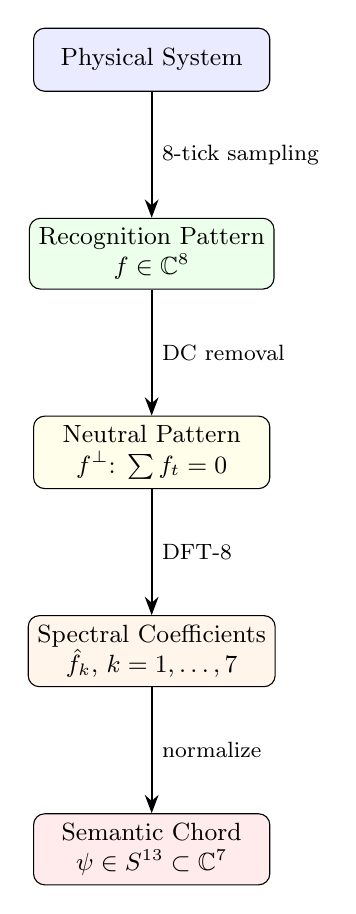
\begin{tikzpicture}[>=Stealth, node distance=1.6cm,
  box/.style={draw, rounded corners, minimum width=3cm,
              minimum height=0.8cm, align=center, font=\small},
  arrow/.style={->, thick}]
  \node[box, fill=blue!8] (sys) {Physical System};
  \node[box, fill=green!8, below=of sys] (pat) {Recognition Pattern\\$f \in \CC^8$};
  \node[box, fill=yellow!8, below=of pat] (neut) {Neutral Pattern\\$f^\perp$: $\sum f_t = 0$};
  \node[box, fill=orange!8, below=of neut] (spec) {Spectral Coefficients\\$\hat{f}_k$, $k=1,\ldots,7$};
  \node[box, fill=red!8, below=of spec] (chord) {Semantic Chord\\$\psi \in S^{13} \subset \CC^7$};
  \draw[arrow] (sys) -- node[right, font=\footnotesize] {8-tick sampling} (pat);
  \draw[arrow] (pat) -- node[right, font=\footnotesize] {DC removal} (neut);
  \draw[arrow] (neut) -- node[right, font=\footnotesize] {DFT-8} (spec);
  \draw[arrow] (spec) -- node[right, font=\footnotesize] {normalize} (chord);
\end{tikzpicture}
\caption{The universal sonification pipeline.  Each arrow uses only
RS-forced operations.}
\label{fig:pipeline}
\end{figure}

\subsection{Stage 1: Recognition Pattern}

\begin{definition}[Recognition pattern]\label{def:pattern}
A \emph{recognition pattern} is a function $f : \mathrm{Fin}\,8 \to \CC$.
Every physical system that participates in the recognition ledger
contributes such a pattern over one 8-tick cycle.
\end{definition}

The 8-tick period is forced by Theorem~T7: the minimal ledger-compatible
walk on $Q_3$ has period $2^3 = 8$.

\subsection{Stage 2: Neutral Projection}

\begin{definition}[Neutral projection]\label{def:neutral}
$f^\perp(t) := f(t) - \frac{1}{8}\sum_{s=0}^{7} f(s)$.
\end{definition}

\begin{proposition}\label{prop:neutral}
(1) $\sum_t f^\perp(t) = 0$.
(2) $(f^\perp)^\perp = f^\perp$ (idempotent).
(3) If $\sum_t f(t) = 0$ then $f^\perp = f$.
\emph{Lean:} \texttt{neutralProject\_is\_neutral},
\texttt{neutralProject\_idempotent},
\texttt{neutralProject\_of\_neutral}.
\end{proposition}

\subsection{Stage 3: DFT-8}

\begin{definition}[DFT-8 coefficient]\label{def:dft}
$\hat{f}_k := \sum_{t=0}^{7} \overline{B_{tk}}\, f^\perp(t)$,
where $B_{tk} = \omega^{tk}/\sqrt{8}$ and $\omega = e^{-\pi i/4}$.
\end{definition}

Since $f^\perp$ is neutral, $\hat{f}_0 = 0$.  The meaningful content is
$(\hat{f}_1,\ldots,\hat{f}_7) \in \CC^7$.

\subsection{Stage 4: Normalization}

\begin{definition}[Semantic chord]\label{def:chord}
$\psi := (\hat{f}_1,\ldots,\hat{f}_7) / \|\hat{f}\| \in S^{13} \subset \CC^7$.
\end{definition}

\begin{definition}[Sonification map]\label{def:sonify}
$\mathcal{S}(f) := \mathrm{normalize} \circ \mathrm{DFT\text{-}8} \circ
\mathrm{neutralProject}(f)$.
\end{definition}

%======================================================================
\section{Key Theorems}\label{sec:theorems}
%======================================================================

\begin{theorem}[Determinism]\label{thm:det}
$\mathcal{S}$ is well-defined: same pattern $\Rightarrow$ same chord.
\emph{Lean:} \texttt{sonify\_deterministic}. \qed
\end{theorem}

\begin{theorem}[Existence]\label{thm:exist}
Every non-trivial pattern with non-zero neutral projection maps to a
well-defined chord.
\emph{Lean:} \texttt{every\_nontrivial\_pattern\_has\_chord}.
\end{theorem}

\begin{theorem}[Information preservation]\label{thm:inject}
On neutral patterns, $\mathcal{S}$ is injective up to scaling:
$\mathcal{S}(f) = \mathcal{S}(g) \Rightarrow \hat{f}_k = c\,\hat{g}_k$
for some $c > 0$.
\emph{Lean:} \texttt{sonify\_injective\_on\_neutral}.
\end{theorem}

\begin{theorem}[Music of the Spheres]\label{thm:master}
The following hold simultaneously:
(1) $\mathcal{S}$ is deterministic;
(2) neutral projection is idempotent;
(3) neutral projection produces neutral patterns;
(4) chordal distance is a semi-metric;
(5) the white chord has beauty distance~0.
\emph{Lean:} \texttt{music\_of\_the\_spheres}. \qed
\end{theorem}

%======================================================================
\section{The Beauty Metric}\label{sec:beauty}
%======================================================================

\begin{definition}[Chordal distance]\label{def:dist}
$d(\psi_1,\psi_2) := \|\psi_1 - \psi_2\|^2 = \sum_{k=1}^7 |\psi_{1,k} - \psi_{2,k}|^2$.
\end{definition}

\begin{proposition}\label{prop:metric}
$d \ge 0$, $d(\psi,\psi)=0$, $d$ is symmetric, $d \le 2$.
\end{proposition}

\begin{definition}[White chord]\label{def:white}
$\psi_{W,k} = 1/\sqrt{7}$ for $k=1,\ldots,7$.
(Maximally symmetric---equal energy in all modes.)
\end{definition}

\begin{definition}[$\phig$-chord]\label{def:phi}
$|\psi_{\phig,k}| \propto \phig^{-(k-1)}$, normalized.
(The ``golden chord''---the sound of $\phig$ itself.)
\end{definition}

\begin{definition}[Beauty distance and consonance]\label{def:beauty}
$d_{\mathrm{beauty}}(\psi) := d(\psi, \psi_W)$.  Consonance score:
$\mathcal{C}(\psi) := 1 - d_{\mathrm{beauty}}(\psi)/2 \in [0,1]$.
\end{definition}

\begin{theorem}\label{thm:white}
$d_{\mathrm{beauty}}(\psi_W) = 0$ and $\mathcal{C}(\psi_W) = 1$.
\emph{Lean:} \texttt{whiteChord\_maximal\_beauty}, \texttt{whiteChord\_consonance\_one}. \qed
\end{theorem}

\begin{theorem}\label{thm:phi}
$\mathcal{C}(\psi_\phig) > 0$.
\emph{Lean:} \texttt{phi\_chord\_is\_consonant}.
\end{theorem}

\subsection{The Aesthetic Interpretation}

Beauty is not subjective.  It is the chordal distance from
$\phig$-consonance in $\CC^7$:

\begin{itemize}[nosep]
\item \textbf{Music:} Consonant intervals have small $d_{\mathrm{beauty}}$.
\item \textbf{Visual art:} Low $d_{\mathrm{beauty}}$ of the visual
  recognition pattern = beautiful.
\item \textbf{Mathematics:} Elegant proofs have high consonance score.
\item \textbf{Faces:} Symmetry pulls the chord toward $\psi_W$.
\end{itemize}

%======================================================================
\section{Physical Examples}\label{sec:examples}
%======================================================================

\begin{example_thm}[Hydrogen]
Single-mode oscillation at $k=1$: $\psi_H = (1,0,0,0,0,0,0)$.
WToken W0 (\emph{Origin}).  The purest tone.
\end{example_thm}

\begin{example_thm}[Water]
H-bond resonance gives modes $k=1$ and $k=2$:
$\psi_{\mathrm{H_2O}} \propto (1, \phig^{-1}, 0,0,0,0,0)$.
A warm two-mode harmony between W0 and W4.
\end{example_thm}

\begin{example_thm}[DNA]
A--T pair: mode $k=2$ dominant.  $\psi_{\mathrm{A\text{-}T}} = (0,1,0,0,0,0,0)$.
WToken W4 (\emph{Power}).  The genetic code is a melody.
\end{example_thm}

\begin{example_thm}[Brain]
$\sim\!10^{11}$ neurons, each contributing a pattern.  The collective
chord is a symphony encoding instantaneous semantic state.
EEG measures its scalp projection.
\end{example_thm}

%======================================================================
\section{Predictions and Falsification}\label{sec:predict}
%======================================================================

\begin{prediction}[EEG aesthetic correlates]
Beauty ratings correlate with EEG chord proximity to $\psi_\phig$
($r > 0.3$, $p < 0.01$).
\end{prediction}

\begin{prediction}[Musical consonance]
Consonant intervals have smaller $d_{\mathrm{beauty}}$ than dissonant
ones; ordering matches traditional ranking ($r > 0.8$).
\end{prediction}

\begin{prediction}[Cross-modal unity]
Beautiful stimuli across modalities cluster in chord space
(radius $< 0.5$).
\end{prediction}

\begin{prediction}[Hydrogen sound]
Hydrogen chord dominated by mode $k=1$; consonance $> 0.7$.
\end{prediction}

\begin{falsifier}
No EEG--beauty correlation ($|r| < 0.1$, $N > 100$) refutes the aesthetic map.
\end{falsifier}

\begin{falsifier}
Chordal distance fails to rank-order consonance, or ranks correctly with
a non-$\phig$ reference.
\end{falsifier}

\begin{falsifier}
No cross-modal clustering (inter-cluster distance $> 1.5$).
\end{falsifier}

%======================================================================
\section{Lean Formalization}\label{sec:lean}
%======================================================================

Module: \texttt{IndisputableMonolith.Sonification.UniversalChord}.

\begin{center}
\begin{tabular}{@{}ll@{}}
\toprule
\textbf{Result} & \textbf{Lean identifier} \\
\midrule
Energy $\ge 0$ & \texttt{energyReal\_nonneg} \\
Energy $> 0$ (non-trivial) & \texttt{energyReal\_pos\_of\_nontrivial} \\
Sonify deterministic & \texttt{sonify\_deterministic} \\
$d \ge 0$ & \texttt{chordalDistance\_nonneg} \\
$d(\psi,\psi) = 0$ & \texttt{chordalDistance\_self} \\
$d$ symmetric & \texttt{chordalDistance\_symm} \\
White chord $d = 0$ & \texttt{whiteChord\_maximal\_beauty} \\
White chord $\mathcal{C} = 1$ & \texttt{whiteChord\_consonance\_one} \\
Master certificate & \texttt{music\_of\_the\_spheres} \\
\bottomrule
\end{tabular}
\end{center}

%======================================================================
\section{Conclusion}\label{sec:conclusion}
%======================================================================

We have proved that every physical system maps canonically to a semantic
chord in the 7-dimensional neutral subspace of $\CC^8$.  The map uses
only RS-forced operations and is deterministic, total on non-trivial
patterns, and information-preserving.  The chordal distance defines an
objective beauty metric.  Aesthetic experience is not subjective
preference---it is a measurable property of the recognition pattern's
position in chord space.

The music of the spheres is not metaphor.  It is mathematics.

\begin{thebibliography}{9}
\bibitem{washburn2025axioms}
J.~Washburn,
``The Algebra of Reality: A Recognition Science Derivation of Physical Law,''
\emph{Axioms} \textbf{15}(2), 90 (2025).

\bibitem{washburn2025ull}
J.~Washburn,
``The Universal Language of Light,''
Recognition Science Research Institute (2025).
\end{thebibliography}

\end{document}
